% LTeX: language=de-CH

\section{Ein eigener Zugang – methodisch und angewandt} \label{sec:methodik}

Dieses Kapitel verortet den methodischen Ansatz dieser Arbeit innerhalb bestehender Konzepte situativer Datenerhebung. Im Zentrum steht dabei die Einordnung der verwendeten Erhebungslogik im Spannungsfeld zwischen \acrfull{esm}, \acrfull{ema} und \acrfull{gema}. Aufbauend auf dieser begrifflichen Abgrenzung werden bestehende digitale Werkzeuge vorgestellt, die vergleichbare Ziele verfolgen. Die vergleichende Analyse dient dazu, Gemeinsamkeiten, Unterschiede und Leerstellen zu identifizieren, um den eigenen methodischen Zugang im Anschluss klar positionieren zu können.

Die konkreten technischen und inhaltlichen Umsetzungen – etwa die Entwicklung der App (\cref{sec:entwicklung_app}) oder die Gestaltung des Fragebogens (\cref{sec:fragebogenentwicklung}) – werden in den folgenden Kapiteln ausführlich dargestellt.


\subsection{Situationen erfassen – Wiederholte Befragung mit \acrshort{esm}, \acrshort{ema} und \acrshort{gema}}

Die systematische Erhebung von affektivem Wohlbedinden erfordert Methoden, die subjektive Erfahrungen möglichst unmittelbar und kontextspezifisch erfassen. Retrospektive Selbstauskünfte sind hierfür nur begrenzt geeignet, da sie Verzerrungen durch selektive Erinnerung oder nachträgliche Neubewertung unterliegen (\textit{Recall Bias}) \parencite{kahnemanDevelopmentsMeasurementSubjective2006}. Um solche Verzerrungen zu vermeiden, wurde bereits in den 1980er-Jahren die \acrfull{esm} entwickelt. Dieses Verfahren basiert auf der mehrfach wiederholten Erhebung subjektiver Zustände im Alltag – etwa durch zeitlich zufällig verteilte Aufforderungen an Teilnehmende, ihre momentane Stimmung, Tätigkeit oder Umgebung zu protokollieren \parencite{csikszentmihalyiValidityReliabilityExperienceSampling1987}. Ziel ist es, das Erleben möglichst nah am Zeitpunkt der Erfahrung und im natürlichen Kontext zu erfassen.

Während \acrshort{esm} ursprünglich als psychologisches Messinstrument konzipiert war, wurde der Ansatz in den 1990er-Jahren durch das Konzept der \acrfull{ema} methodologisch erweitert. \acrshort{ema} bezeichnet nicht nur die unmittelbare Erhebung subjektiven Erlebens, sondern schliesst auch physiologische, verhaltensbezogene oder kontextuelle Daten mit ein – etwa über mobile Geräte, Sensorik oder Tagebuchsysteme \parencite{shiffmanEcologicalMomentaryAssessment2008}. Der Begriff „ecological“ verweist hierbei nicht auf natürliche Umwelt, sondern auf den Anspruch, Erleben und Verhalten im realweltlichen Lebenskontext zu erfassen.

Mit der zunehmenden Verbreitung von GPS-fähigen Endgeräten wurde \acrshort{ema} in den 2010er-Jahren durch das Konzept der \acrfull{gema} ergänzt. \acrshort{gema} kombiniert die subjektive Momentaufnahme mit objektiven, räumlich verortbaren Kontextinformationen wie Standort, Wetter, Lärm oder Bebauungsstruktur \parencite{kirchnerSpatiotemporalDeterminantsMental2016}. Im Unterschied zu \acrshort{ema} liegt der Fokus hier auf der systematischen räumlichen Verknüpfung: Subjektive Erfahrungen werden nicht nur als situativ, sondern explizit als räumlich situiert begriffen. Entscheidend ist dabei nicht die Art der Umgebung – also ob es sich etwa um Grünflächen, urbane Plätze oder Transiträume handelt –, sondern die Möglichkeit, affektives Erleben in seiner Beziehung zum jeweils spezifischen räumlich-materiellen Kontext zu analysieren.

Die vorliegende Arbeit folgt diesem methodischen Paradigma. Ziel ist es, situativ affektive Zustände im Raum nicht nur als individuelle, sondern als kontextuell-räumlich bedingte Erfahrungen zu erfassen. Zu diesem Zweck wurde eine eigene Smartphone-Applikation (\textit{InterMind}) entwickelt, die Teilnehmende mehrmals täglich dazu auffordert, eine kurze Selbsteinschätzung ihres momentanen Wohlbefindens und ihrer Umgebung vorzunehmen. Gleichzeitig werden automatisiert Geodaten gespeichert, sodass jede Beobachtung in ihrer konkreten räumlichen Verortung analysiert werden kann. Im Unterschied zu vielen bestehenden \acrshort{gema}-Studien liegt der Fokus dabei nicht auf spezifischen Umweltmerkmalen wie Vegetationsanteil oder Luftqualität, sondern auf der relationalen Analyse von Raum und subjektivem Erleben.

Die Entscheidung für ein solches Studiendesign bringt gegenüber querschnittbasierten Verfahren mehrere methodische Vorteile mit sich. Erstens reduziert die wiederholte intraindividuelle Erhebung Verzerrungen durch retrospektive Einschätzungen und erlaubt eine präzisere Erfassung situativer Schwankungen \parencite{randallDevelopmentTrialMobile2013}. Zweitens ermöglicht sie eine Kontrolle individueller Basisniveaus, was insbesondere für intersektionale Analysen relevant ist, die sowohl zwischen als auch innerhalb von Personen Differenzierungen vornehmen. Drittens erlaubt die Kombination von Echtzeitbefragung und Geodatenanalyse eine kontextsensitive Modellierung der Beziehungen zwischen affektivem Zustand und Umgebung – im Sinne eines relationalen, ökologisch verstandenen Raumbegriffs \parencite{mascherekMeadowsAsphaltRoad2025}.


\subsection{Anknüpfen und Abgrenzen – Vergleich mit bestehenden Instrumenten}

Die im Rahmen dieser Arbeit entwickelte App bewegt sich im Spannungsfeld zweier methodischer Herangehensweisen: der Echtzeiterhebung räumlich kontextualisierter affektiver Zustände (wie bei \textit{Urban Mind}) und der explizit intersektionalen Analyse subjektiver Raumwahrnehmungen (wie bei \textit{Relief Maps+}). Beide bestehenden Instrumente bilden wichtige Referenzpunkte, da sie jeweils zentrale Teilaspekte des hier verfolgten Ansatzes adressieren, jedoch keine vollständige Integration beider Perspektiven vornehmen. Der folgende Vergleich dient dazu, methodische Gemeinsamkeiten und Unterschiede herauszuarbeiten.

\subsubsection*{Urban Mind: \acrshort{gema} ohne intersektionale Perspektive}

Das \textit{\gls{urbanmind}}-Projekt\footnote{Siehe \href{https://www.urbanmind.info/}{urbanmind.info}} stellt ein beispielhaftes Werkzeug dar, um subjektives momentanes Wohlbefinden in städtischen Kontexten mittels Echtzeiterhebungen systematisch zu erfassen und zu analysieren \parencite{bakolisUrbanMindUsing2018}. Es basiert auf einer mobilen Smartphone-App, die mithilfe von \acrshort{gema} detaillierte Einblicke in den Zusammenhang zwischen unmittelbaren Umweltfaktoren und psychischer Gesundheit ermöglicht.

Zentrales Anliegen des \textit{Urban Mind}-Tools ist es, die Effekte spezifischer natürlicherElemente der Umgebung, wie beispielsweise Bäume, Himmel, Wasser oder Vogelgesang, auf die psychische Gesundheit in Echtzeit zu untersuchen. Hierfür werden Proband\genderstern innen mehrmals täglich über einen Zeitraum von zwei Wochen aufgefordert, kurze standardisierte Fragen zu ihrer aktuellen Umgebung und ihrem momentanen Wohlbefinden zu beantworten \parencite{bakolisUrbanMindUsing2018}. Die Datenerhebung erfolgt sowohl mittels Selbsteinschätzungen der räumlichen und sozialen Umgebung als auch über Geodaten, welche automatisiert die exakte räumliche Verortung der Teilnehmer\genderstern innen ermöglichen.

\begin{figure}[h]
    \centering
    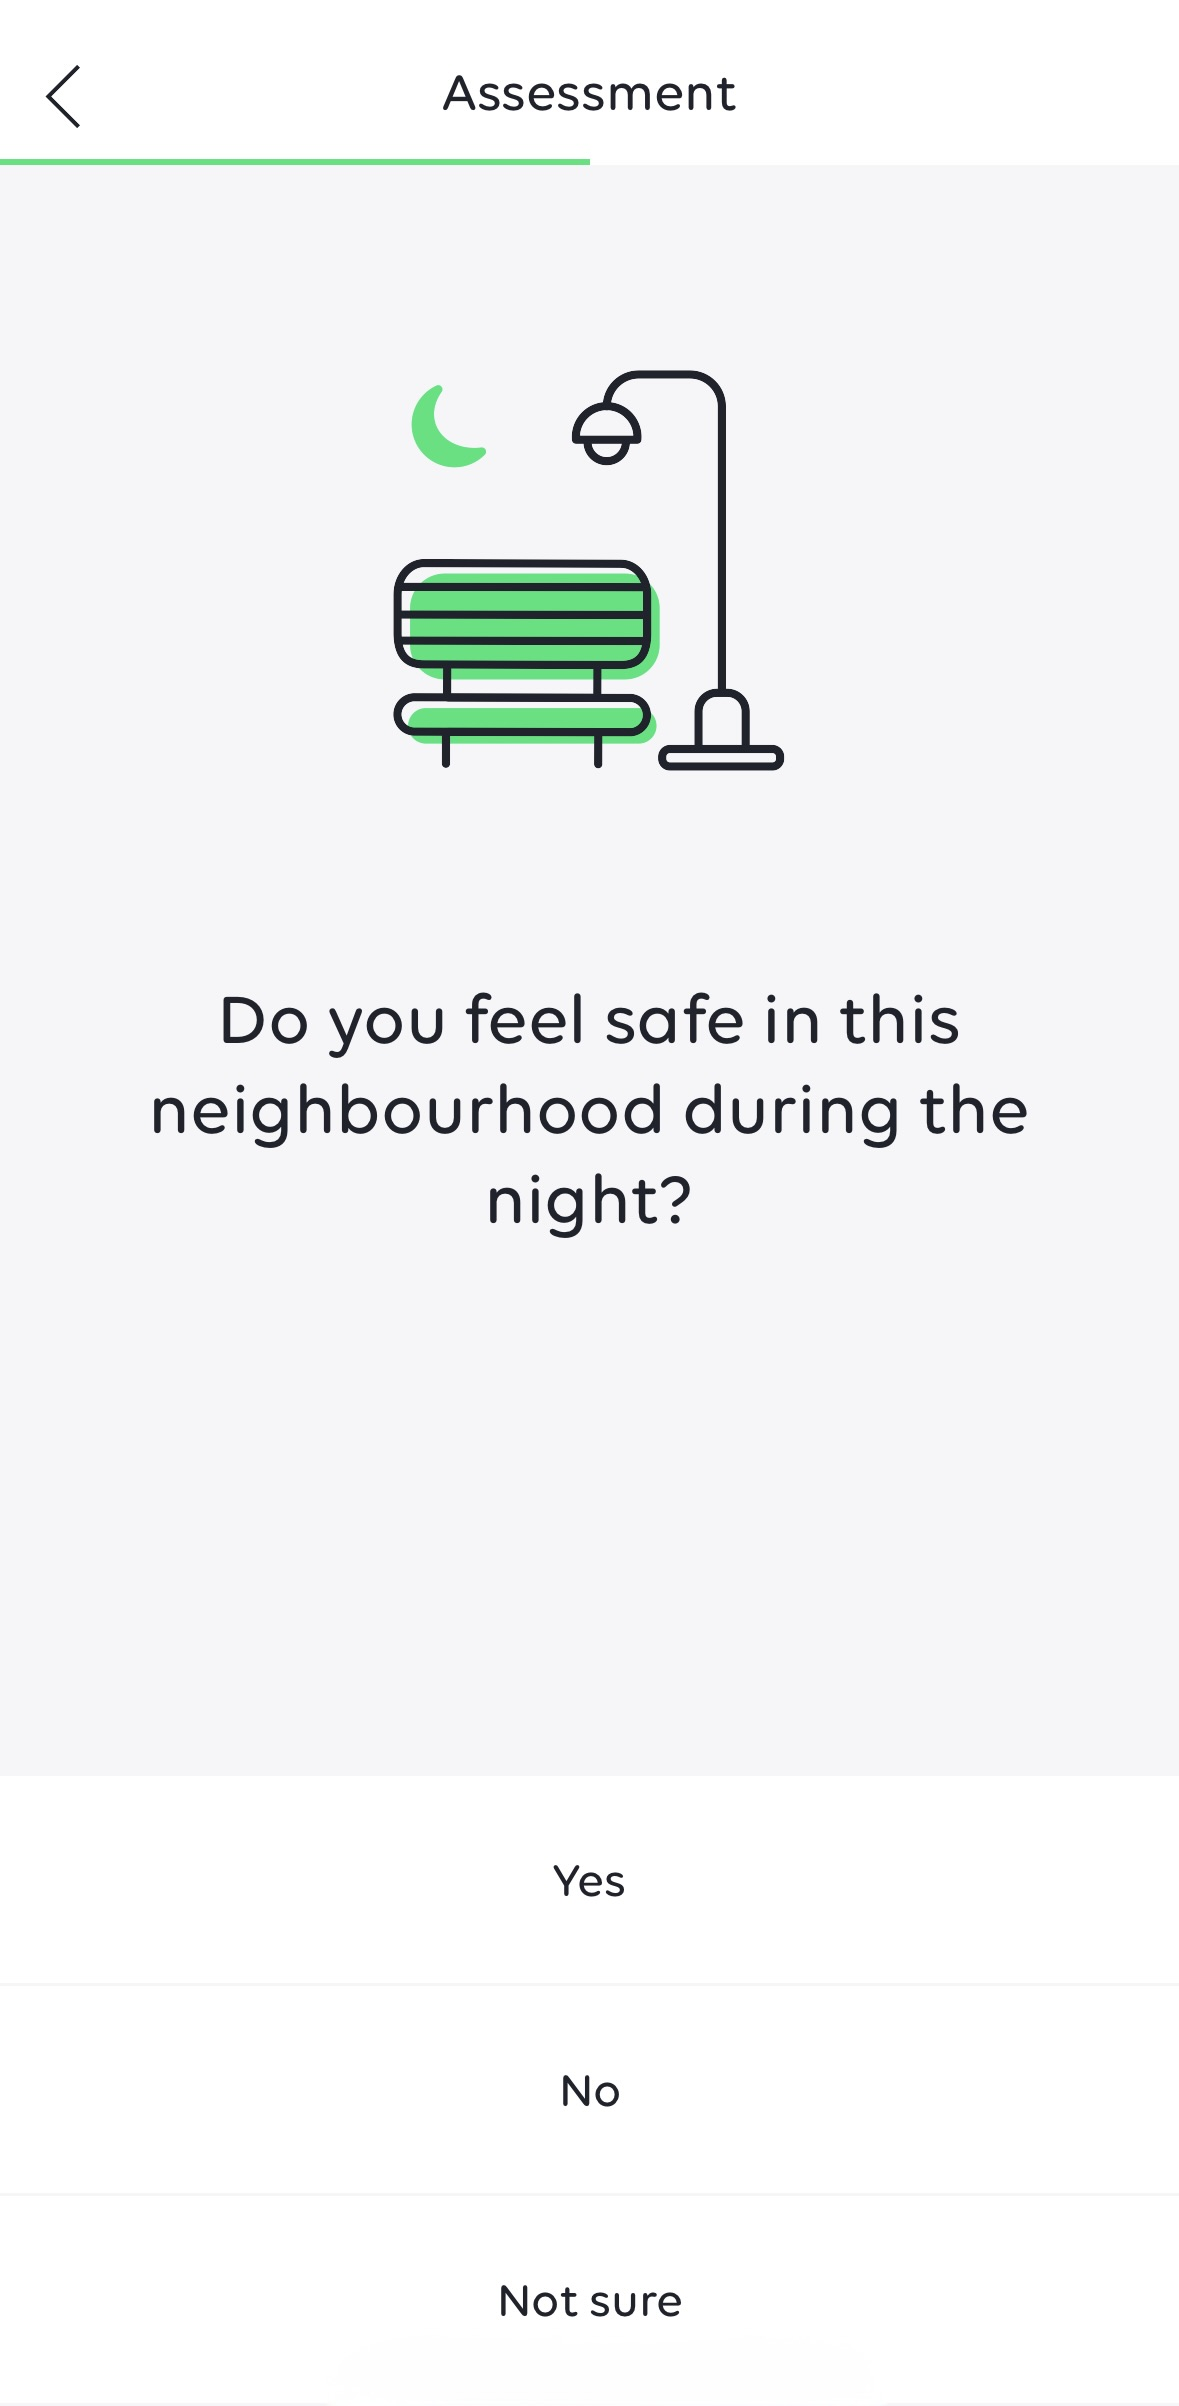
\includegraphics[width=0.3\textwidth]{Arbeit/images/urban_mind01.jpeg}
    \caption{Screenshot einer typischen Frageseite aus der Urban Mind-App}
    \label{fig:urban_mind_screenshot_1}
\end{figure}

Im Gegensatz zu traditionellen querschnittlichen Designs erlaubt das Urban Mind-Tool explizit die Analyse unmittelbarer und zeitverzögerter Effekte (Lag-Effekte). So konnten beispielsweise signifikant positive Effekte von natürlichen Elementen wie Vogelgesang oder dem Vorhandensein von Bäumen auf das momentane Wohlbefinden nachgewiesen werden, welche auch mehrere Stunden nach dem eigentlichen Kontakt noch messbar waren \parencite{bakolisUrbanMindUsing2018}. Darüber hinaus betont das Tool die Bedeutung individueller Differenzen und psychologischer Charakteristika, wie beispielsweise Impulsivität, die sich als moderierende Variable herausstellte: Personen mit höherer Impulsivität, welche typischerweise ein erhöhtes Risiko für psychische Erkrankungen aufweisen, profitieren stärker von unmittelbaren Naturerfahrungen.

Hinsichtlich des Designs und der Bedienbarkeit überzeugt die Urban Mind-App durch eine intuitive grafische Gestaltung (siehe \Cref{fig:urban_mind_screenshot_1}) sowie durch motivierende Elemente wie eine visuelle Übersicht über ausgefüllte und verpasste Fragebögen. Zudem ermöglicht sie Nutzer\genderstern innen, ihre eigenen Daten retrospektiv aufzubereiten, was zu einer angeleiteten Reflexion des eigenen Wohlbefindens beiträgt. Dieses Feature unterstützt insbesondere eine nachhaltige und motivierte Teilnahme über den gesamten Erhebungszeitraum hinweg.

Obwohl Urban Mind zahlreiche methodische und technische Stärken aufweist, berücksichtigt es intersektionale Perspektiven bisher nicht explizit. So sind beispielsweise soziale Kategorien wie Geschlecht, Ethnizität oder sozioökonomischer Status zwar als demografische Variablen erfasst, werden jedoch nicht systematisch in einer intersektionalen Analyse miteinander in Beziehung gesetzt. Theoretisch wäre es möglich, intersektionale Analysen retrospektiv auf Grundlage der erhobenen Daten durchzuführen, eine solche methodische Perspektive wurde jedoch bislang nicht verfolgt.

\subsubsection*{Relief Maps+: Reflexive und intersektionale Kartierung retrospektiver Erfahrungen}

Im Unterschied zu Echtzeit-Tools wie „Urban Mind“, die affektives Wohlbefinden situativ-erlebensnah quantifizieren, verfolgt \textit{\gls{reliefmaps}}\footnote{Siehe \href{https://reliefmaps.upf.edu/}{reliefmaps.upf.edu}} einen qualitativ-reflexiven Ansatz, der retrospektiv subjektive Erfahrungen intersektional positioniert sichtbar macht \parencite{rodo-de-zarateDevelopingGeographiesIntersectionality2014}. Aufbauend auf der ursprünglichen Version der „Relief Maps“ integriert die digitale Anwendung drei miteinander verschränkte Dimensionen – geografische Orte, soziale Identitäten und emotionale Bewertungen – und legt dabei besonderen Wert auf die Förderung individueller Selbstreflexion und kollektiver Sichtbarmachung diskriminierender Raumstrukturen.

Zu Beginn des Erhebungsprozesses erstellen Nutzer\genderstern innen einen Avatar auf Basis intersektional relevanter Merkmale wie Geschlecht, Sexualität, Klasse, Herkunft, Körperbild oder (Dis-)Ability. Darauf aufbauend reflektieren sie in mehreren Schritten über emotionale Erfahrungen in verschiedenen Raumkategorien wie „öffentliche Räume“, „Gesundheitseinrichtungen“ oder „virtuelle Räume“ (siehe \cref{fig:relief_maps_plus_screenshot_1}). Für jede Achse sozialer Positionierung können in einem nächsten Schritt Orte je nach erfahrenem (Un-)Wohlsein als unterdrückend, kontrovers, neutral oder entlastend klassifiziert werden. Ergänzend können Orte direkt auf einer Karte verortet und mit freien Kommentaren sowie Emotionslabels wie „Angst“, „Sicherheit“ oder „Empowerment“ versehen werden. Diese Funktion fördert eine dichte, kontextualisierte Beschreibung subjektiver Erlebnisse, die sich nicht auf standardisierte Itemskalen reduzieren lässt.

\begin{figure}[htbp]
    \centering
    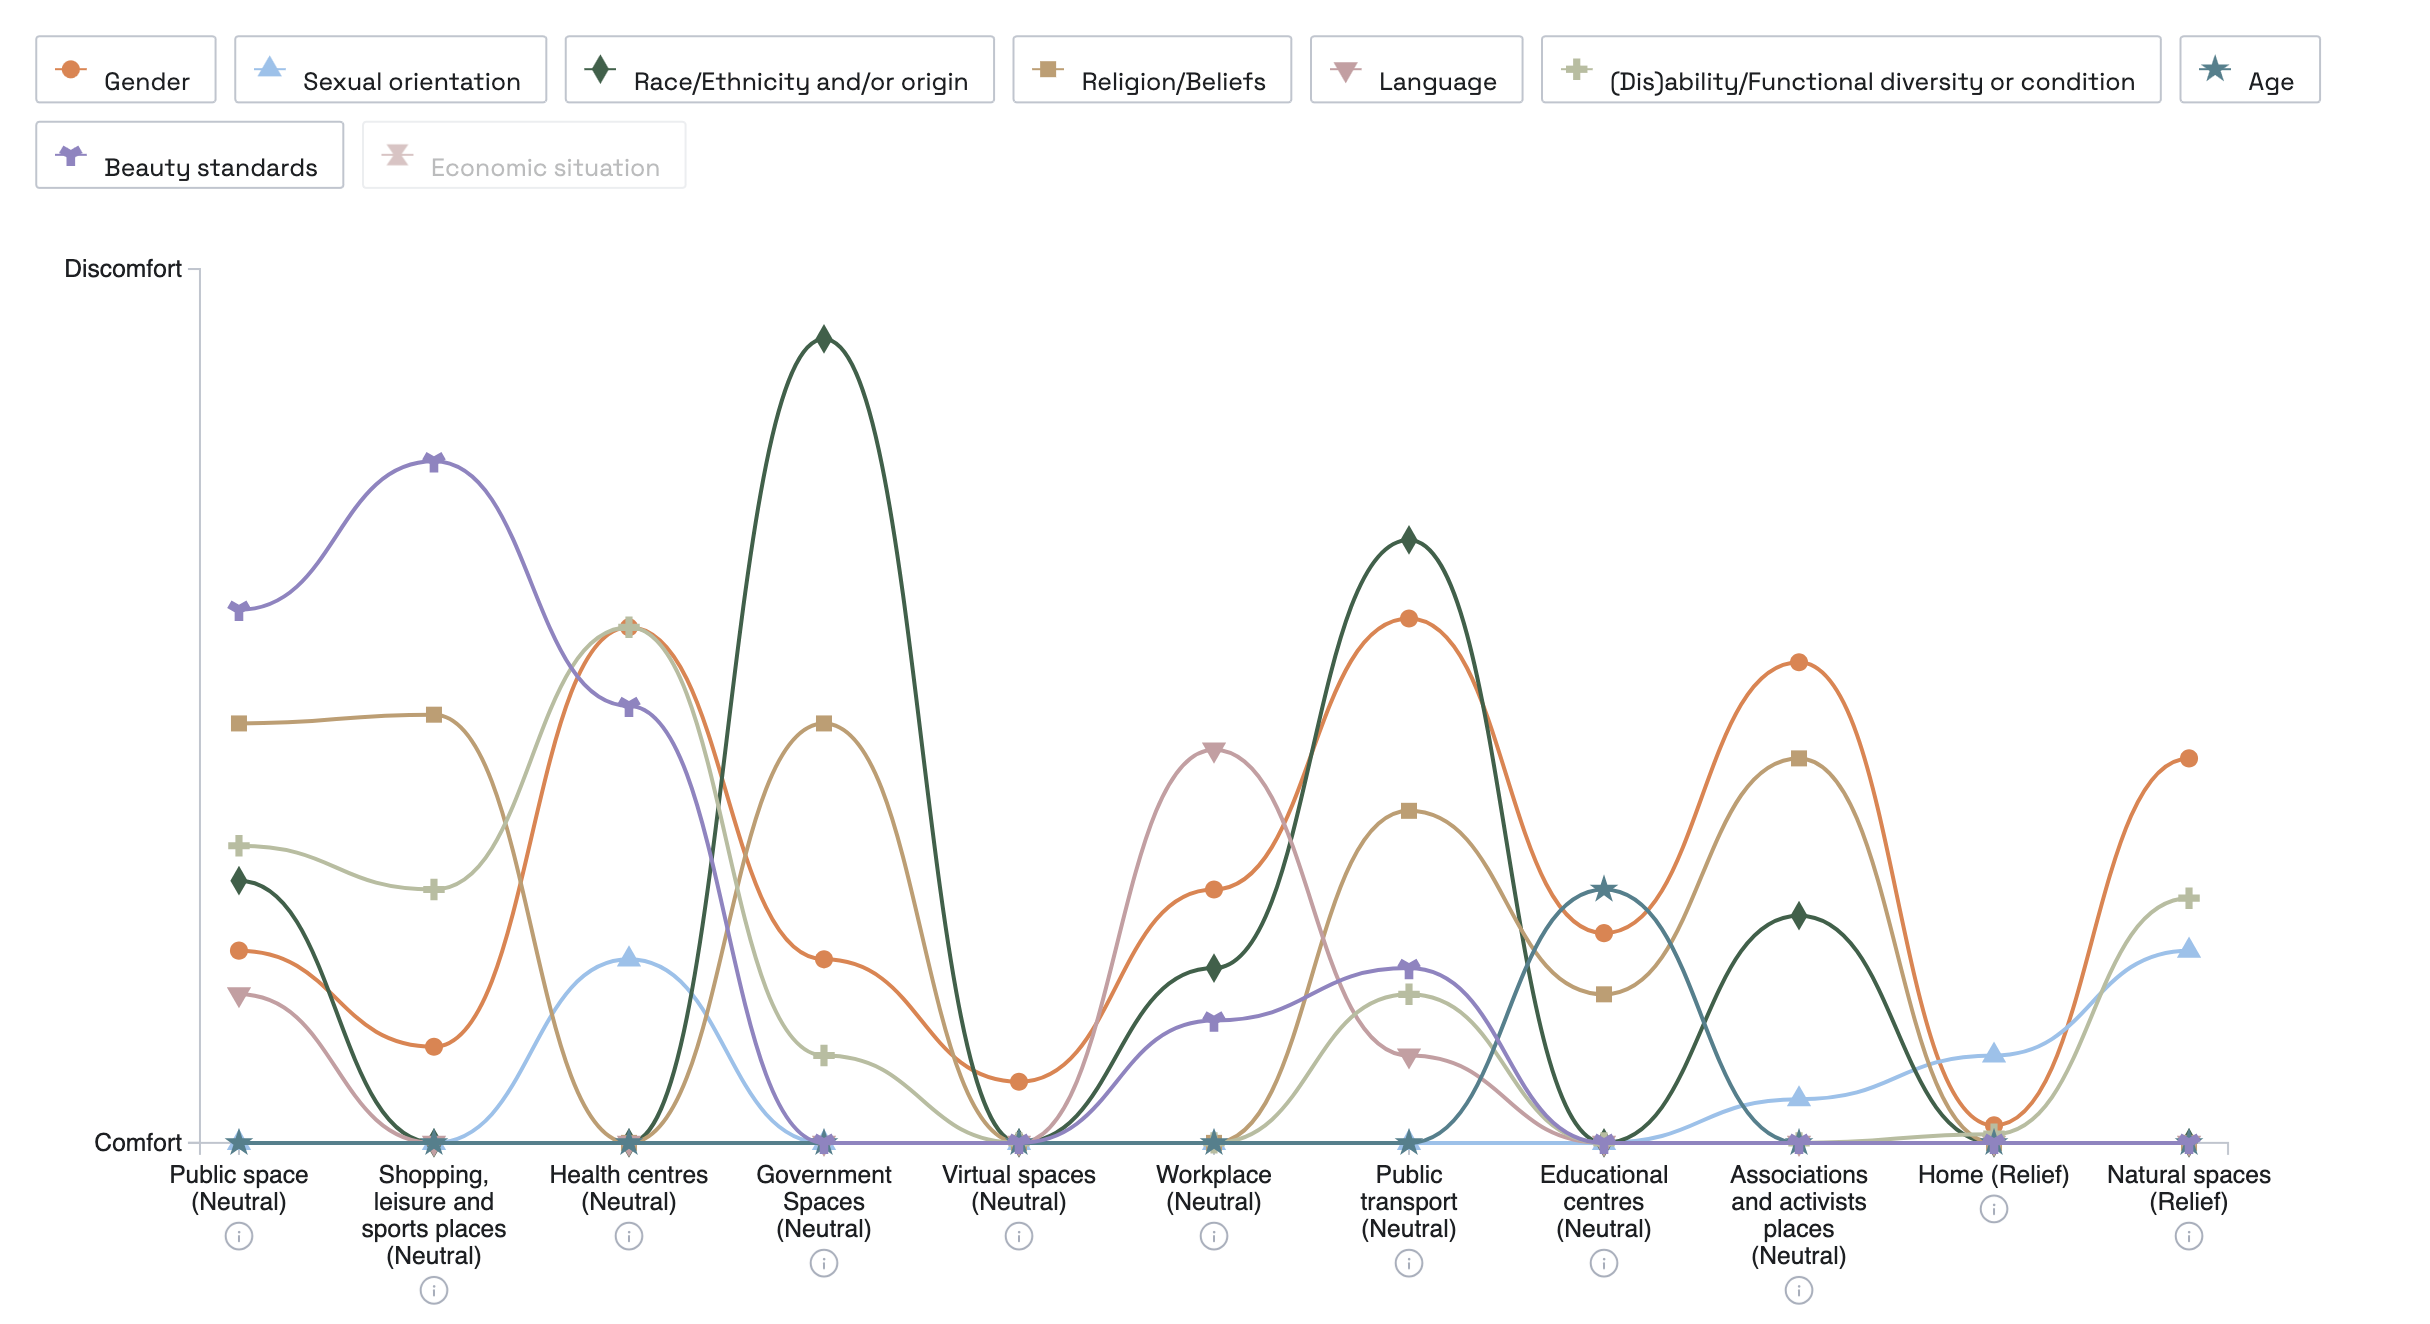
\includegraphics[width=\textwidth]{Arbeit/images/reliefmap.png}
    \caption{Beispielhafte Ausgabe aus dem Relief Maps+ Tool}
    \label{fig:relief_maps_plus_screenshot_1}
\end{figure}

Ein zentrales methodisches Merkmal von Relief Maps+ ist der Versuch, die emotionale Wirkung sozialer Machtverhältnisse räumlich darstellbar zu machen – ohne diese in eindimensionale Kausalbeziehungen zu überführen. Die Nutzer\genderstern innen bewerten ihre Erfahrungen explizit entlang einzelner \glspl{identitaetsachse}. Gleichzeitig zeigt sich hier eine zentrale methodologische Spannung: Die isolierte Betrachtung einzelner Diskriminierungsachsen widerspricht dem Grundgedanken intersektionaler Analyse, der gerade auf die Verwobenheit und Gleichzeitigkeit verschiedener Machtverhältnisse verweist. Eine konsequente intersektionale Operationalisierung bleibt damit methodisch herausfordernd.

Einige technische Merkmale von Relief Maps+ sind auch im Hinblick auf die Entwicklung eigener Tools relevant. Die browserbasierte Anwendung erlaubt es Forschenden, eigenständig Projekte zu erstellen und auszuwerten. Allerdings ist der Zugang derzeit stark auf den katalanischen Kontext zugeschnitten: Verfügbare Sprachen sind Katalanisch, Spanisch und Englisch; Optionen zur Erweiterung oder Lokalisierung sind nicht dokumentiert. Da der Quellcode nicht öffentlich zugänglich ist, bleiben Fragen zur Anpassbarkeit, Wiederverwendbarkeit und langfristigen Wartbarkeit offen. Aus methodischer Sicht stellt sich somit die Frage, inwiefern die Software übertragbar ist auf andere sprachliche, kulturelle und geografische Kontexte.

Trotz dieser Einschränkung eröffnet Relief Maps+ wichtige Potenziale: Die bewusste Integration von Reflexivität, die aktive Beteiligung der Nutzer\genderstern innen an der Interpretation ihrer eigenen Erfahrungen sowie die Sichtbarmachung räumlich kontextualisierter Ungleichheiten markieren einen innovativen Zugang für intersektionale, subjektzentrierte Geographien. Die methodische Fundierung des Tools beruht auf einem iterativen Validierungsprozess unter Einbezug feministischer, queerer und dekolonialer Perspektiven \parencite{luizdesouzaSpiralValidationProcess2025}.



\subsection{Mehr Infrastruktur als Innovation}

Die im Rahmen dieser Arbeit entwickelte App \textit{InterMind} versteht sich als offen zugängliches und flexibel einsetzbares Werkzeug für Studien im Rahmen der \acrshort{gema}. Ziel war es, eine technisch eigenständige, quelloffene Infrastruktur bereitzustellen, die eine situative, geolokalisierte Erhebung affektiven Wohlbefindens ermöglicht – ein Instrument, das in dieser Form bislang nicht allgemein verfügbar war. Die Entwicklung orientierte sich in Teilen an bestehenden Tools wie \textit{Urban Mind}, insbesondere was das Interface-Design und die Nutzerführung betrifft, basiert jedoch auf einer unabhängig konzipierten Codebasis und wurde vollständig neu implementiert.

Die App selbst ist methodisch nicht innovativ im engeren Sinne, sondern stellt eine robuste, anpassbare Plattform dar, die für verschiedenste \acrshort{gema}-Studien konfiguriert werden kann. Ihr modularer Aufbau erlaubt die Integration beliebiger Fragebögen und Fragetypen – einschliesslich Freitextfeldern, Schiebereglern oder Mehrfachantworten. Damit kann das System flexibel an unterschiedliche Forschungskontexte angepasst und in zukünftigen Studien weiterverwendet werden.

Im Zentrum der vorliegenden Arbeit steht ein spezifisch entwickelter Fragebogen, der auf der App zum Einsatz kommt. Dieser kombiniert klassische \gls{ema}-Items zur situativen Erfassung von Kontext und Wohlbefinden mit explizit intersektional angelegten Fragen. Dabei werden Dimensionen wie Geschlecht, Herkunft oder sozioökonomischer Status getrennt erfasst – ein Ansatz, der zwar theoretisch nicht vollständig der Idee intersektionaler Verwobenheit entspricht, aber eine quantitative Auswertbarkeit ermöglicht. Gleichzeitig bleibt durch offene Antwortformate Raum für reflexive Auseinandersetzung mit der eigenen Erfahrung in konkreten räumlichen Situationen.

